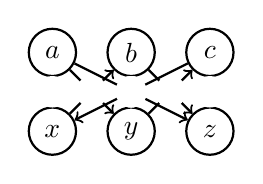
\begin{tikzpicture}[->, thick, main/.style = {circle,draw, inner sep = 0pt, minimum size = 0.6cm}, edge/.style = {circle, midway, fill=white, inner sep=0pt, minimum size=0.4cm}, scale = 0.5]    \node[main] (a) at (0, 0) {$a$};
    \node[main] (b) at (2, 0) {$b$};
    \node[main] (c) at (4, 0) {$c$};
    \node[main] (x) at (0, -2) {$x$};
    \node[main] (y) at (2, -2) {$y$};
    \node[main] (z) at (4, -2) {$z$};
    \path
        (a) edge[bend right = 0] node[edge] {} (x)
        (a) edge[bend right = 0] node[edge] {} (y)
        (x) edge[bend right = 0] node[edge] {} (b)
        (b) edge[bend right = 0] node[edge] {} (y)
        (y) edge[bend right = 0] node[edge] {} (c)
        (b) edge[bend right = 0] node[edge] {} (z)
        (c) edge[bend right = 0] node[edge] {} (z)
        (a) edge[bend right = 0] node[edge] {} (z)
        (c) edge[bend right = 0] node[edge] {} (x);
\end{tikzpicture}